\documentclass[11pt, letterpaper]{article}
\usepackage[margin=1in]{geometry}
\usepackage[style=apa]{biblatex}
\usepackage{setspace}
\usepackage{amsmath}
\usepackage{amssymb}
\usepackage{bm}
\usepackage{graphicx}
\linespread{1.5}

\title{A Joint Model for Item Response and Process}
\author{Xiang Liu}
\date{\today}

\addbibresource{lit.bib}
\begin{document}
	\maketitle
  \section{Introduction}
  For a very long time, educational researchers often have to make certain
  compromise in studying human behavior between on large scale and in fine
  detail. For example, in a 1992 study \parencite{Pinnell1995}, National Assessment of
  Educational Progress (NAEP), the largest nationally representative and
  continuing assessment of grade students, was interested in measuring
  students' oral reading fluency which may provide an informative window into
  their process of reading \parencite{Bergner2018}. A representative sample of
  $1,136$ fourth-grade students who participated in the reading assessment
  that year were initially selected to work with the interviewer and read
  aloud a brief passage as a screening task with a more difficult assessment
  passage followed up in the same interview. The entire process was
  audio-taped and later analyzed. The data collected is much richer and
  potentially more informative than the responses to the traditional reading
  comprehension tasks alone. However, both the data collection process as well
  as the  analysis procedure are labor-intensive and expensive. As a result,
  it is difficult to scale up. In fact, the 1992 study was considered large
  scale of its time. Advance in technology leads to new possibilities. More
  recently, In
  2002, a NAEP special study again focused on oral reading fluency 
  \parencite{Daane2005}. The design was very similar to the decade old study.
  However, instead of audio-taping, the 2002 study involved the
  computer-assisted collection and digital recording. 

  Fast forward almost two decades. Explosion in technological innovation
  touches every corner of our society and brings us into the Big Data era.
  Fields of educational research are no exception. The Big Data offers
  unprecedented opportunities for tracking and analyzing behavior 
  \parencite{Markowetz2014}. For instance, in 2017, NAEP mathematics and reading
  assessments were transitioning to be digitally based for grades 4 and 8.
  Instead of the
  traditional paper-and-pencil assessments, the national assessment began to
  be administered on digital mobile devices (i.e. tablets with an attached
  keyboard, stylus, and earbuds). Not only the modality of the test
  administration changed, more importantly, authentic items have been
  developed and used in the assessment. Examples include the
  scenario-based-tasks (SBT) from the technology and engineering literacy
  (TEL; \cite{TheNationalCenterforEducationStatistics2013}) assessment where
  students are asked to interact with items in an interactive multimedia
  environment \parencite{Hao2015}. Furthermore, the digital assessment platform
  allows collection of process data produced from students' interaction with
  the digital assessment platform.

  The emergence of the big data presents new opportunities. In addition to the
  traditional item responses, granular process data are now available at
  large scale to educational researchers and practitioners. Potentially,
  the collected process data may be utilized to improve the measurement of
  the relevant constructs and/or provide more detailed individualized
  feedback to students and teachers. But, at the same time, extracting useful
  information and making sound inferences from these complex and statistically
  noisy large-scale data poses serious methodological challenges. 

  \section{Research goals}
  The behaviors captured in the process data may relate to both item response
  and proficiency. The additional information from process data could prove to
  be useful in improving measurement precision as well as leading to better
  understanding the cognitive process of students. However, to achieve these, we
  need to develop modeling approaches that could simultaneously consider item
  response and process data.

  \section{Methods}
  In this section, we briefly introduce the proposed latent variable model.
  Without loss of generality, we consider the case of dichotomous item
  response and some dichotomous behavior from process. Let random variables $X_
  {ij}$, $i = 1, 2, \dots, N$ and $j = 1, 2, \dots, J$ denote the item response
  from the $i$th student to the $j$th item. $X_{ij} = 1$ if the response is
  correct, and $X_{ij} = 0$ if incorrect. Similarly, let $W_{ij}$ denote a
  dichotomous behavior captured during the response process. One example of the
  dichotomous behavior could be calculator usage, i.e. $W_{ij} = 1$ if the $i$th
  student used the on-screen calculator for the $j$th item, $W_{ij} = 0$
  otherwise. To model $\bm{X}$ and $\bm{W}$ jointly, we propose a
  multi-dimensional latent variable model. $W_{ij}$ is conditionally independent
  from each other given the latent propensity $\theta_{i2}$ and parameters
  $\alpha_j$ and $\beta_j$. And the probability of $W_{ij} = 1$ is given by a
  two-parameter logistic (2PL) model, i.e.
  \begin{equation}
    P(W_{ij} = 1 | \theta_{i2}, \alpha_j, \beta_j) = \frac{\exp[\alpha_j 
    (\theta_{i2} - \beta_j)]}{1 + \exp[\alpha_j (\theta_{i2} - \beta_j)]}.
  \end{equation}
  The item response $X_{ij}$ does not only depend on the student's
  proficiency $\theta_{i1}$ and item parameters $a_j$ and $b_j$, but potentially
  also on $w_{ij}$ and some effect $\gamma_j$. The probability of a correct
  response is given by
  \begin{equation}
    P(X_{ij} = 1 | \theta_{i1}, a_j, b_j, w_{ij}, \gamma_j) = \frac{\exp[a_j
    (\theta_{i1} - b_j + w_{ij} \gamma_j)]}{1 + \exp[a_j(\theta_{i1} - b_j + w_
    {ij} \gamma_j)]}.
  \end{equation}
  Furthermore, we allow the two latent variables, $\bm{\theta}_i = (\theta_{i1},
  \theta_{i2})$, to be correlated through a multivariate normal distribution
  centered at the origin with a unit scale and a correlation $\rho$,
  \begin{equation}
    \bm{\theta}_i \sim \Phi\left(\bm{0}, 
    \begin{bmatrix}
    1 & \rho \\
    \rho & 1 \\
    \end{bmatrix}\right).
  \end{equation}
  Therefore, marginalizing $\bm{\theta}_i$ over the multivariate normal
  distribution function $\Phi$, the joint probability of observing $\bm{X}_i = 
  (x_{i1}, x_{i2}, \dots, x_{iJ})$ and $\bm{W}_i = (w_{i1}, w_{i2}, \dots, w_
  {iJ})$ is
  \begin{gather}
  \begin{aligned}
    &P(\bm{X}_i = \bm{x}_i, \bm{W}_i = \bm{w}_i | \bm{a}, \bm{b}, \bm{\alpha}, 
    \bm{\beta}, \bm{\gamma}, \rho)\\ &= \iint \limits_{\bm{\theta}_i \in 
    \mathbb{R}^2} \prod_{j = 1}^{J} P(X_{ij} = x_{ij} | \theta_{i1}, a_j, b_j, w_
    {ij}, \gamma_j)P(W_{ij} = w_{ij} | \theta_{i2}, \alpha_j, \beta_j) d\Phi
    (\bm{\theta}_i;\rho)
  \end{aligned}
  \end{gather}
  Figure \ref{fig:latent_variable_model} shows the graphical representation of
  the model.
  \begin{figure}
  \label{fig:latent_variable_model}
  \centering
    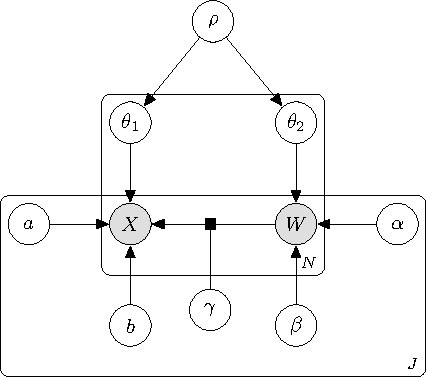
\includegraphics[scale = 1.0]{figure/joint_model_diagram.pdf}
    \caption{A probabilistic graphical model representation}
  \end{figure}

  \section{Proposed Work}
  In this project, we plan to develop statistical methods for this new class of
  latent variable models as described in the previous section for the purpose of
  joint modeling of item response and process data. Specifically, we will
  \begin{itemize}
    \item develop and implement an expectation-maximization (EM) algorithm for
    finding the maximum likelihood estimates (MLE);

    \item study the procedures for approximating the covariance matrix of the MLE
    so that realistic standard errors of parameter estimates can be quickly
    obtained;

    \item develop methods for evaluating aspects of model fit, such as the
    overall goodness-of-fit, person-level fit, and item-level fit;

    \item fit the real NAEP datasets and possibly modify the model according to
    the results;

    \item compare the estimated student proficiency from joint model to that of
    the IRT model without process data;

    \item disseminate the results through manuscripts and presentations.
  \end{itemize}

  \section{NAEP dataset}
  The project is methodological in nature; however, we'll demonstrate the
  utility of the methods by fitting the model on a real NAEP dataset. We plan to
  use the 2017 Math assessment released blocks. For these items, we'll build a
  dataset consisting scored item responses as well as the on-screen calculator
  usage from process data. We will also consider datasets involve other tool
  usage, such as the text-to-speech. No identifiable information will be used.

  \section{Discussion}
  The proposed model can be understood as a variation of multidimensional item
  response theory (MIRT) models. In fact, if the tool effects $\gamma_j = 0$,
  $\forall j$, the model reduces to a MIRT model with a simple structure.
  However, modeling the direct effect between process behavior and item response
  is crucial. While a student's proficiency level could affect the process
  behaviors through correlations between latent variables, we would expect
  different process behaviors would affect the probability of getting an item
  correct directly in addition to through the correlated latent variables. For
  example, two students with the same level of math proficiency could have
  different chances of answering a particular item correctly if one of them used
  calculator and the other did not due to the different levels of cognitive
  difficulties involved.

  The model is relatively simple and could be adapted for the joint modeling of
  different forms of process data and item response.

  \section{Schedule, staffing, and budget}
  We plan to implement the study from May to October 2020. Below is the
  estimated hours for project members:
  \begin{itemize}
    \item Xiang Liu - 240 hours
    \item Jie Gao   - 100 hours
    \item Matt Johnson - 20 hours
    \item Data analysts and others - 40 hours
    \item Total - 400 hours
  \end{itemize}
 


  \newpage
  \printbibliography
\end{document}